% ==============================================
% !TEX root = ./critics.tex
% ==============================================
% ==============================================
\section{Motivating Examples and Tool Features}
\label{sec:motivation}
% ==============================================
\begin{figure*}
\centering
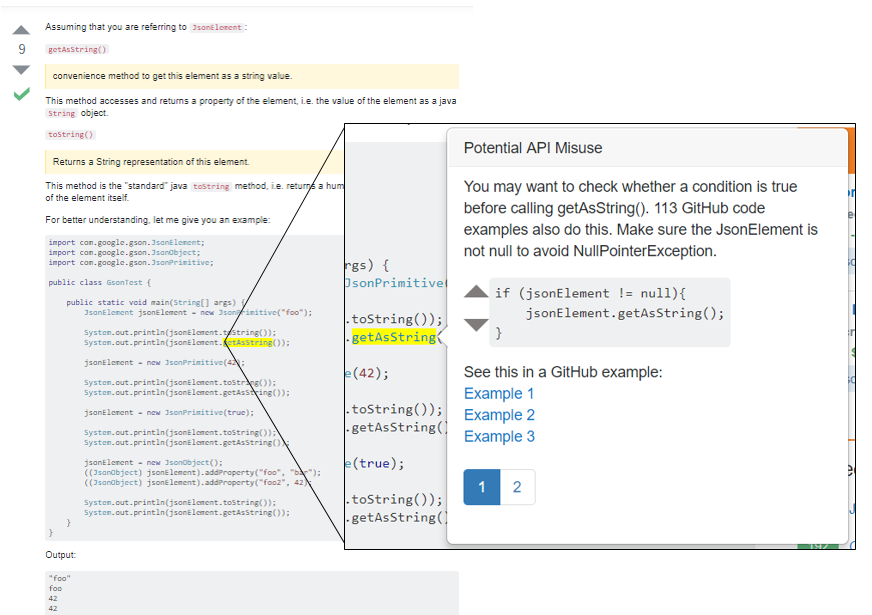
\includegraphics[width=0.6\textwidth]{json_ex1_context.PNG}
  \vspace{.1in}
  \caption{A code snippet that does not properly check {\tt JsonElement.getAsString}.\protect\footnotemark}
  \label{fig:so_example}
\end{figure*}

\begin{figure*}[t!]
\centering
  \begin{subfigure}[t]{0.48\textwidth}
  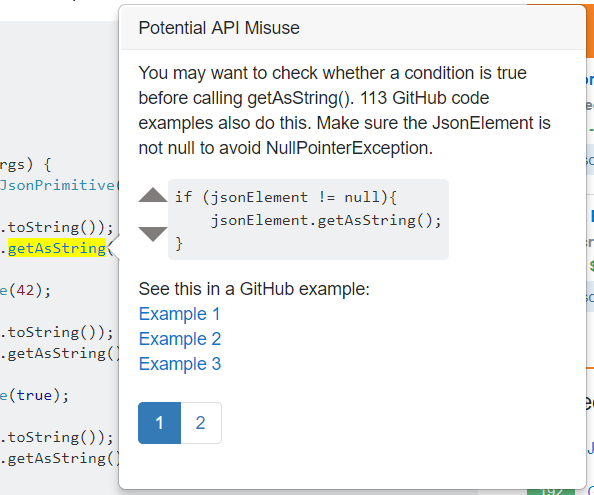
\includegraphics[width=\textwidth, height=6cm]{json_ex2.PNG}
  \caption{A page describing a way to avoid a {\tt NullPointerException} by checking whether the {\tt JsonElement} object is null. \todo{should I still include this figure when it's sort of subsumed by Figure~\ref{fig:so_example}?}} 
  \label{fig:page1}
  \end{subfigure}
  \hspace{0.02\textwidth}
  \begin{subfigure}[t]{0.48\textwidth}
  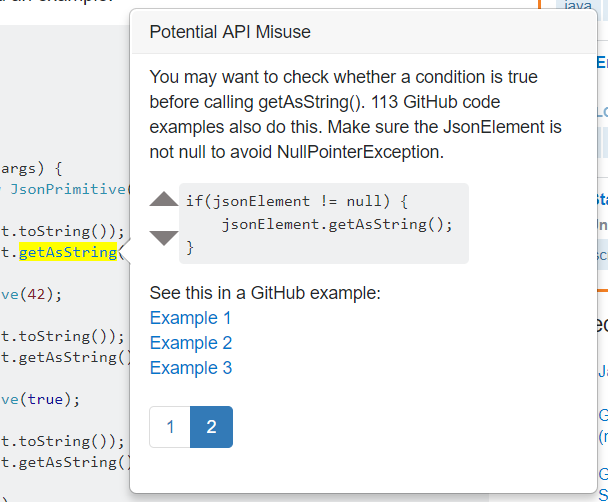
\includegraphics[width=\textwidth, height=6cm]{json_ex3.PNG}
  \caption{A page describing a way to avoid a {\tt ClassCastException} by checking whether the {\tt JsonElement} object is a primitive.}
  \label{fig:page2}
  \end{subfigure}
  \hfill
  \vspace{0.02\textwidth}
\caption{The two pages of a popup generated on {\tt JsonElement.getAsString}.\todo{Can we also show how many users like or dislike the violations in the popup window? Since we don't have any real users, maybe we need to create some artificial numbers for the demonstration purpose.}}
\label{fig:features}
\end{figure*}

\footnotetext{https://stackoverflow.com/questions/34120882/gson-jsonelement-getasstring-vs-jsonelement-tostring}

Consider Alice, a software developer who needs to convert Java objects to their JSON representations using Google's Gson library\footnote{https://github.com/google/gson/blob/master/UserGuide.md}, which she is unfamiliar with. Alice finds a Stack Overflow post that demonstrates how to get the string value of a json element, as shown in Figure~\ref{fig:so_example}. However, this example does not use the {\tt JsonElement} API properly. 

{\bf Detecting and Highlighting Potential API Misuse.}
%\todo{Describe briefly the patterns of JsonElement.getAsString like ``The pattern mining technique learns two patterns that are commonly practiced by GitHub developers...'' You can refer to the last paragraph of the motivating example section of our ASE draft.}
The pattern mining technique learns two {\tt JsonElement.getAs\-String} patterns that are commonly practiced by GitHub developers: (1) a check to make sure that the {\tt JsonElement} object is of the type {\tt JsonPrimitive} by using {\tt JsonElement.isJsonPrimitive} before calling {\tt getAsString}, and (2) a check to make sure that the {\tt JsonElement} object is not null before calling {\tt getAsString}.

The extension highlights the potential API misuse in the code snippet, as seen in Figure 2. Alice is interested in learning more about the API and what specifically the code snippet did not include, so she clicks on the highlighted text.

{\bf Stack Overflow Popup View.}
Clicking on the highlighted text reveals a popup, as seen in Figure 2a and 2b. The popup is populated with information about any required patterns in {\soa}'s database this particular API call does not adhere to. Alice notices that there are two pages of the popup, indicating two different usage patterns that this call does not follow, as shown in Figure~\ref{fig:page1} and Figure~\ref{fig:page2}. 

Alice inspects the first page (Figure~\ref{fig:page1}) and sees a warning message, automatically generated by {\soa} for that particular API misuse. She learns that she should check whether the {\tt JsonElement} object is null before calling {\tt getAsString}. She notices that 113 other GitHub code examples use this pattern, which gives her a quantitative measurement of how prevalent this pattern is in real-world projects. Below this is a code example following the required pattern, generated by {\soa} based on the context of the SO example.

Alice then inspects the second page (Figure~\ref{fig:page2}), and finds that it suggests to check whether the {\tt JsonElement} object is primitive before calling {\tt getAsString} to avoid a {\tt ClassCastException}. She notices that this pattern has less than half the support of the previous pattern.

Curious to see the first pattern in context, Alice returns to the first page of the popup and clicks on the first link provided to her under "See this in a GitHub example."

\begin{figure*}[t!]
\centering
  \begin{subfigure}[t]{0.48\textwidth}
  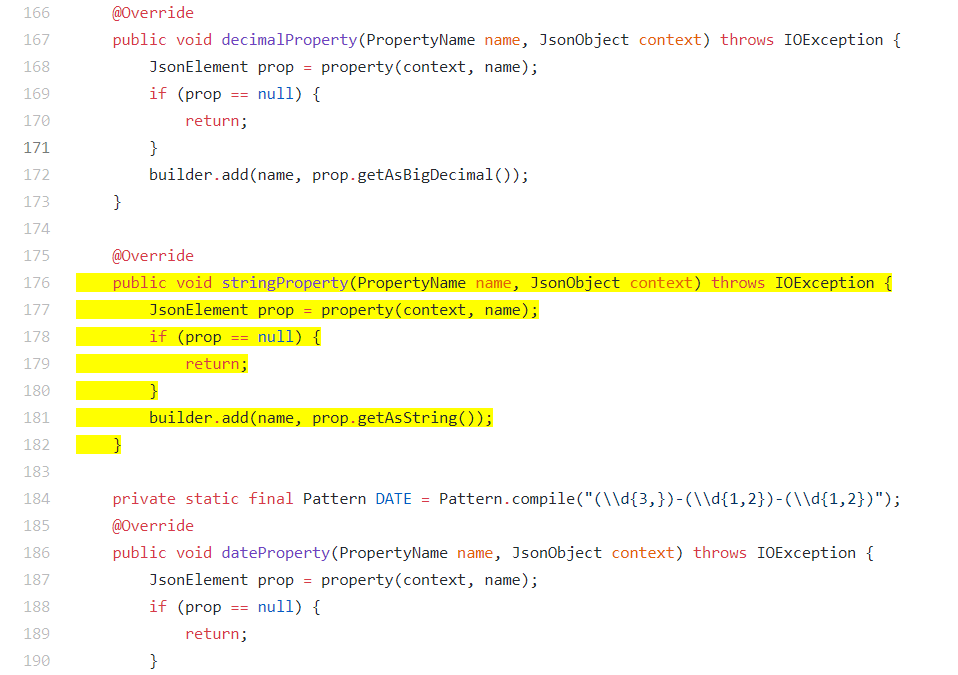
\includegraphics[width=\textwidth]{json_null_gh2_context.PNG}
  \caption{The second GitHub example for Figure~\ref{fig:page1} in the context of its GitHub file.\protect\footnotemark} 
  \vspace{.1in}
  \label{fig:github1}
  \end{subfigure}
  \hfill
  \begin{subfigure}[t]{0.48\textwidth}
  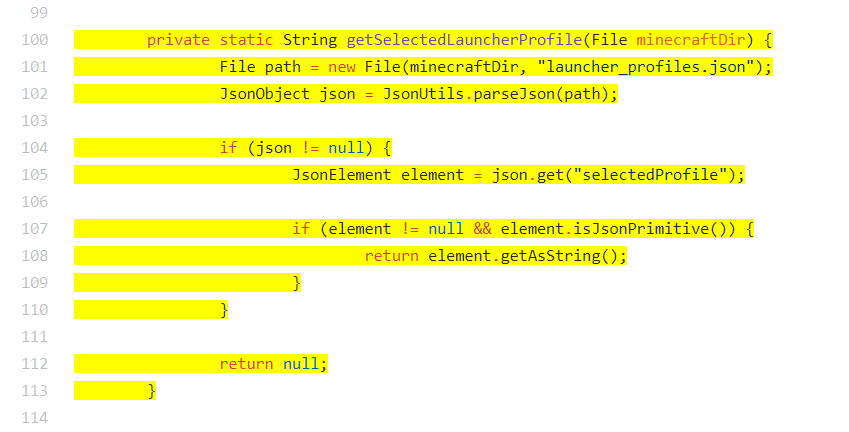
\includegraphics[width=\textwidth]{json_primitive_gh1.PNG}
  \caption{The first GitHub example for Figure~\ref{fig:page2}.\protect\footnotemark}
  \vspace{.1in}
  \label{fig:github2}
  \end{subfigure}
  \hfill
\caption{The GitHub examples redirected to from the links provided in the popup, highlighted by the Chrome extension.\todo{The snapshot only shows the highlighted code. Is there a better way to give paper reviewers some context that the highlighted code is from GitHub and that the code is selectively highlighted by our tool instead of by GitHub?}}
\label{fig:github_examples}
\end{figure*}

%\begin{figure}
%\centering
%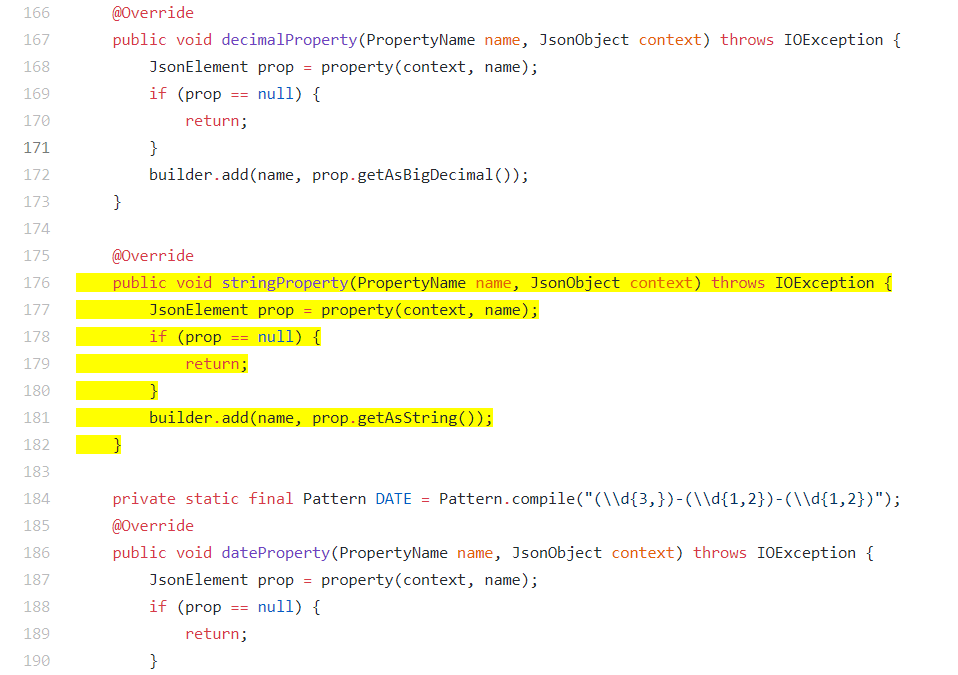
\includegraphics[width=0.48\textwidth]{json_null_gh2_context.PNG}
  %\caption{The GitHub example that a link from Figure~\ref{fig:page1} redirects to, highlighted by the Chrome extension.\protect\footnotemark} 
  %\label{fig:github_examples}
%\end{figure}

{\bf GitHub Example View.} When Alice clicks on one of the GitHub links, the file opens in a new tab and the view scrolls to where the API is called in the file, and the method in which this occurs is highlighted so Alice can easily find it, as seen in Figure~\ref{fig:github_examples}. The addition of a compilable code example that demonstrates the pattern in context can aid Alice in understanding how to use the pattern if it is unfamiliar to her. In this case, Alice finds herself redirected to the method in a GitHub project seen in Figure~\ref{fig:github_examples}.

Returning to the popup in Stack Overflow, Alice clicks on the second link provided for the second page to compare usage patterns in context. This link opens up to the GitHub method seen in Figure~\ref{fig:github2}. She notices that the example uses a null check in conjunction with the primitive check, which makes sense to her after seeing that both were missing from the Stack Overflow code snippet. However, she notes that the more commonly-used pattern only uses a null check.

After seeing these two examples, Alice can infer that a null check is more necessary and is more common than the primitive check, based on the GitHub examples she has seen as well as the GitHub support indicated by the popup message. She upvotes the null check's pattern by clicking on the up-arrow on its page (see Figure~\ref{fig:page2}) to send the server her feedback on the patterns it gave her.

%https://github.com/asakusafw/asakusafw/blob/cad94753128bd3168e23c0539cc55c7e5a653dbd/asakusa-test-data-provider/src/main/java/com/asakusafw/testdriver/json/JsonObjectDriver.java
\footnotetext{http://tinyurl.com/JsonObjectDriver}

%https://github.com/Spoutcraft/Spoutcraft/blob/5cbbc2b07edaf4194a36130a7e74321e5b30ace0/src/main/java/com/prupe/mcpatcher/Config.java
\footnotetext{http://tinyurl.com/SpoutcraftConfig}